\section{\uppercase{Encoding the Dynamics}}
\label{sec:representation-results}

\noindent
Experiments~1 and~2 compare the encodings on common participant partitions, with LPQ extraction and SVM selection held fixed, so that each comparison changes only the image encoding.

\subsection{A Fixed Descriptor for the Comparison}
\label{sec:descriptor}
\noindent
Local Phase Quantization describes texture through local Fourier phase information \cite{Ojansivu2008}, and we apply the same implementation independently to each RGB channel. Its compact phase histograms tolerate blur and are therefore robust to the smoothing introduced by resizing, rasterization and anti-aliasing. This suits minimaps drawn with a fixed line width, where the relevant information lies in the spatial organization of the strokes and in local variations of the semantic channels rather than in stroke thickness. Preliminary comparisons with Local Binary Patterns, GLCM/Haralick statistics, Gabor filters and wavelet features found no alternative consistently superior across tasks.

Before extraction, foreground is detected by any channel intensity below 250. We crop its bounding box, add a margin equal to 5\% of the longer dimension, pad to a square with white, and resize to $64\times64$ by bilinear interpolation. LPQ filters each channel with four complex $5\times5$ kernels; the signs of their real and imaginary responses form an eight-bit code at each pixel, and a 256-bin histogram per channel, normalized by its count and square-rooted element-wise, is concatenated into a 768-attribute vector. The static RGB channels are identical, so the static vector repeats the same histogram three times, which keeps the nominal dimension constant without adding information.

Standardization and support vector machine fitting \cite{Cortes1995} occur inside each training partition, over a 21-candidate search: five linear models with $C\in\{0.01,0.1,1,10,100\}$ and sixteen radial-basis models with $C\in\{0.1,1,10,100\}$ and $\gamma\in\{\mathrm{scale},10^{-4},10^{-3},10^{-2}\}$, with inverse-frequency class weights. The SVM learns from LPQ image texture and receives no original signal measurements as tabular features. Holding the leading encoding and the partitions fixed, it also outperformed regularized logistic regression (0.5674) and a Random Forest \cite{Breiman2001} (0.5599), neither gap surviving correction, and a compact convolutional network trained from scratch on $128\times128$ pixels \cite{LeCun1998} (0.5105), by 0.0646 [0.0277, 0.1021] at adjusted $p=0.0054$, the one contrast of Experiment~1 that survives its family; that last comparison also reflects differences in input resolution and search budget.

\subsection{Single Signals and RGB Combinations}
\label{sec:classifiers}
\begin{figure*}[t]
\centering
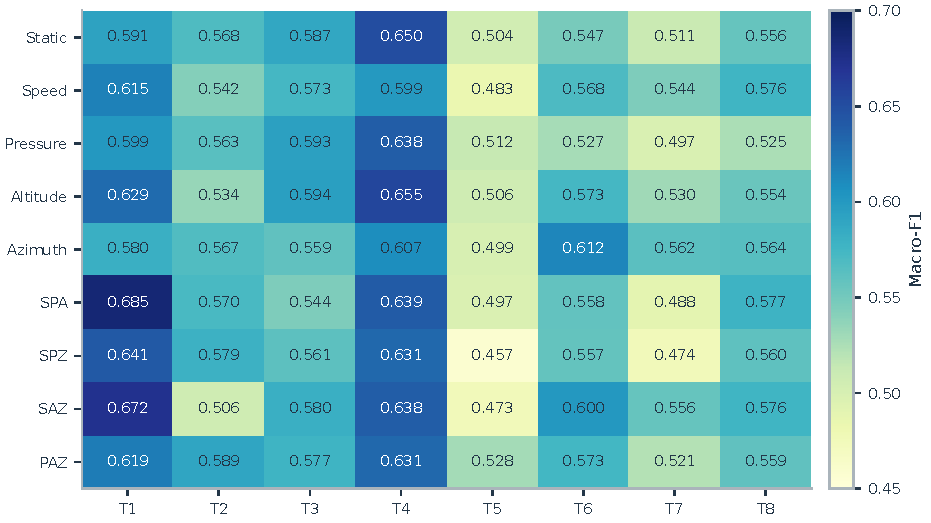
\includegraphics[width=0.58\textwidth]{encoding_heatmap.pdf}
\caption{Recording-level macro F1 of Experiment~1 for every encoding and task, averaged over five repetitions. Rows follow Table~\ref{tab:encoding}. Color helps most on the spiral (T1), and the best encoding differs between tasks.}
\label{fig:heatmap}
\end{figure*}
\noindent
Experiment~1 starts from the static trace (encoding~1), which reaches a recording-level macro F1 of 0.5643 over the eight tasks. Altitude and azimuth are the most informative single signals, at 0.5718 and 0.5688, while speed reaches 0.5625 and pressure 0.5568. Combining three signals gives the best encodings: $SAZ$ (8) reaches 0.5752 and $PAZ$ (9) 0.5746, ahead of $SPA$ (6) at 0.5697 and $SPZ$ (7) at 0.5574. The near tie between $SAZ$ and $PAZ$ suggests that speed and pressure are largely interchangeable alongside the two pen angles, and the paired gain of $SAZ$ over the static trace is +0.0109 [$-$0.0146, 0.0370].

These averages hide a strong dependence on the task (Figure~\ref{fig:heatmap}). Every encoding except azimuth alone raises the spiral above the static trace, where $SAZ$ adds 0.0802 and $SPA$ reaches 0.685 against 0.591; azimuth lifts T6 from 0.547 to 0.612; altitude gives the best T4; $SAZ$ lowers T2 by 0.0612; and T5 remains difficult for every encoding. Because $SAZ$ was chosen as the leading encoding from outer-test scores, Experiment~2 repeats the choice with training participants only.

\subsection{Choosing the Encoding Within Training}
\label{sec:nested-followup}
\noindent
Experiment~2 evaluates the procedure that chooses an encoding. Within each outer training set, each task and encoding receives the same 21-candidate SVM search, and one encoding is chosen for all eight tasks by the unweighted mean of the selected per-task scores, with ties resolved in favor of the static trace. The fusion rule is chosen in the same way, on validation predictions obtained inside the training participants. We compare a fixed static policy, selection among all nine encodings, and selection among the eight dynamic encodings.

Training data consistently favor the dynamics. Although ties went to the static trace, selection among all nine encodings chose a dynamic encoding in 24 of the 25 outer training sets, and no single signal dominates: in the dynamic-only policy, azimuth (5) was chosen five times and $SAZ$ (8) four times. On the recording-level endpoint the dynamic-only policy reaches 0.5643 and the nine-encoding policy 0.5618, against 0.5620 for static, with paired differences of +0.0023 [$-$0.0172, 0.0221] and $-$0.0002 [$-$0.0192, 0.0190]. One encoding chosen for eight heterogeneous tasks averages gains with losses, from +0.0567 on the spiral to $-$0.0274 on T5. With the fusion rule also chosen inside training, participant-level macro F1 is 0.6017 for dynamic-only and 0.5991 for nine-encoding selection, against 0.6171 for static. Experiment~3 therefore tests the selected encoding on a shorter and more homogeneous task set.

\subsection{Controls of the Signal--Position Association}
\label{sec:controls}
\noindent
Adding color changes both the signal content and the image texture. Two controls keep the ingredients of the texture and change only where each signal value occurs: a nonzero circular shift by 25--75\% of the segments within each pen-down stroke, and a joint permutation of the segments within that stroke. The three channels move together, so each segment keeps its combination of values; single-segment strokes are unchanged, no value crosses a pen lift, and geometry, line width and normalization are preserved. Each control transforms training and test recordings with three fixed seeds and repeats the dynamic-only selection; metrics are averaged over seeds, and bootstrap draws keep each participant's tasks, repetitions and seeds together.

Displacing the signals within strokes lowered recording-level macro F1 from 0.5643 to 0.5561 under circular shifts, a decrease of 0.0082 [$-$0.0102, 0.0264], and to 0.5442 under joint permutation, a decrease of 0.0201 [0.0010, 0.0399] whose interval lies above zero. The effect is largest on the spiral, where permutation removes 0.0609 [0.0086, 0.1174]. Performance therefore depends on where the dynamics are placed along the trajectory, not only on the colors present in the image. The four contrasts of this experiment, the two selection policies against static and dynamic-only selection against each control, form one Holm family, in which the permutation effect has adjusted $p=0.1848$; confirming it will require a larger cohort.
